% ==================================================
% CHAPTER 2: Characterization of sTGCs using cosmic rays %
% ==================================================

\chapter{Characterization of sTGCs using cosmic rays}
\label{chap:cosmics}
% Edit count: Lia - 0, Brigitte - 0

In Canada, the cathode boards are prepared at TRIUMF in Vancouver, British Columbia; the quadruplets are constructed at Carleton University in Ottawa, Ontario; and are tested and characterized with cosmic muons at McGill University in Montreal, Quebec. Cosmic muon characterization was done with a typical hodoscope.  The quadruplet was placed in the test bench (of which a complete description can be found in Lefebvre, 2018~\cite{lefebvre_thesis}). Above and below it was a layer of scintillator-PMT arrays, labelled in figure~\ref{fig:hodoscope}. The arrays provided a trigger (using a NIM crate) for cosmic muons when both fired in coincidence. The trigger was passed \iffalse through a KC705\footnote{Xilinx, Xilinx Kintex-7 FPGA KC705 Evaluation Kit, EK-K7-KC705-G, 2018} which sent it \fi to the front end boards attached to the adaptor boards of each layer of the quadruplet to readout the quadruplet. 

\section{Collecting cosmic muon data}
\begin{figure}
    \centering
    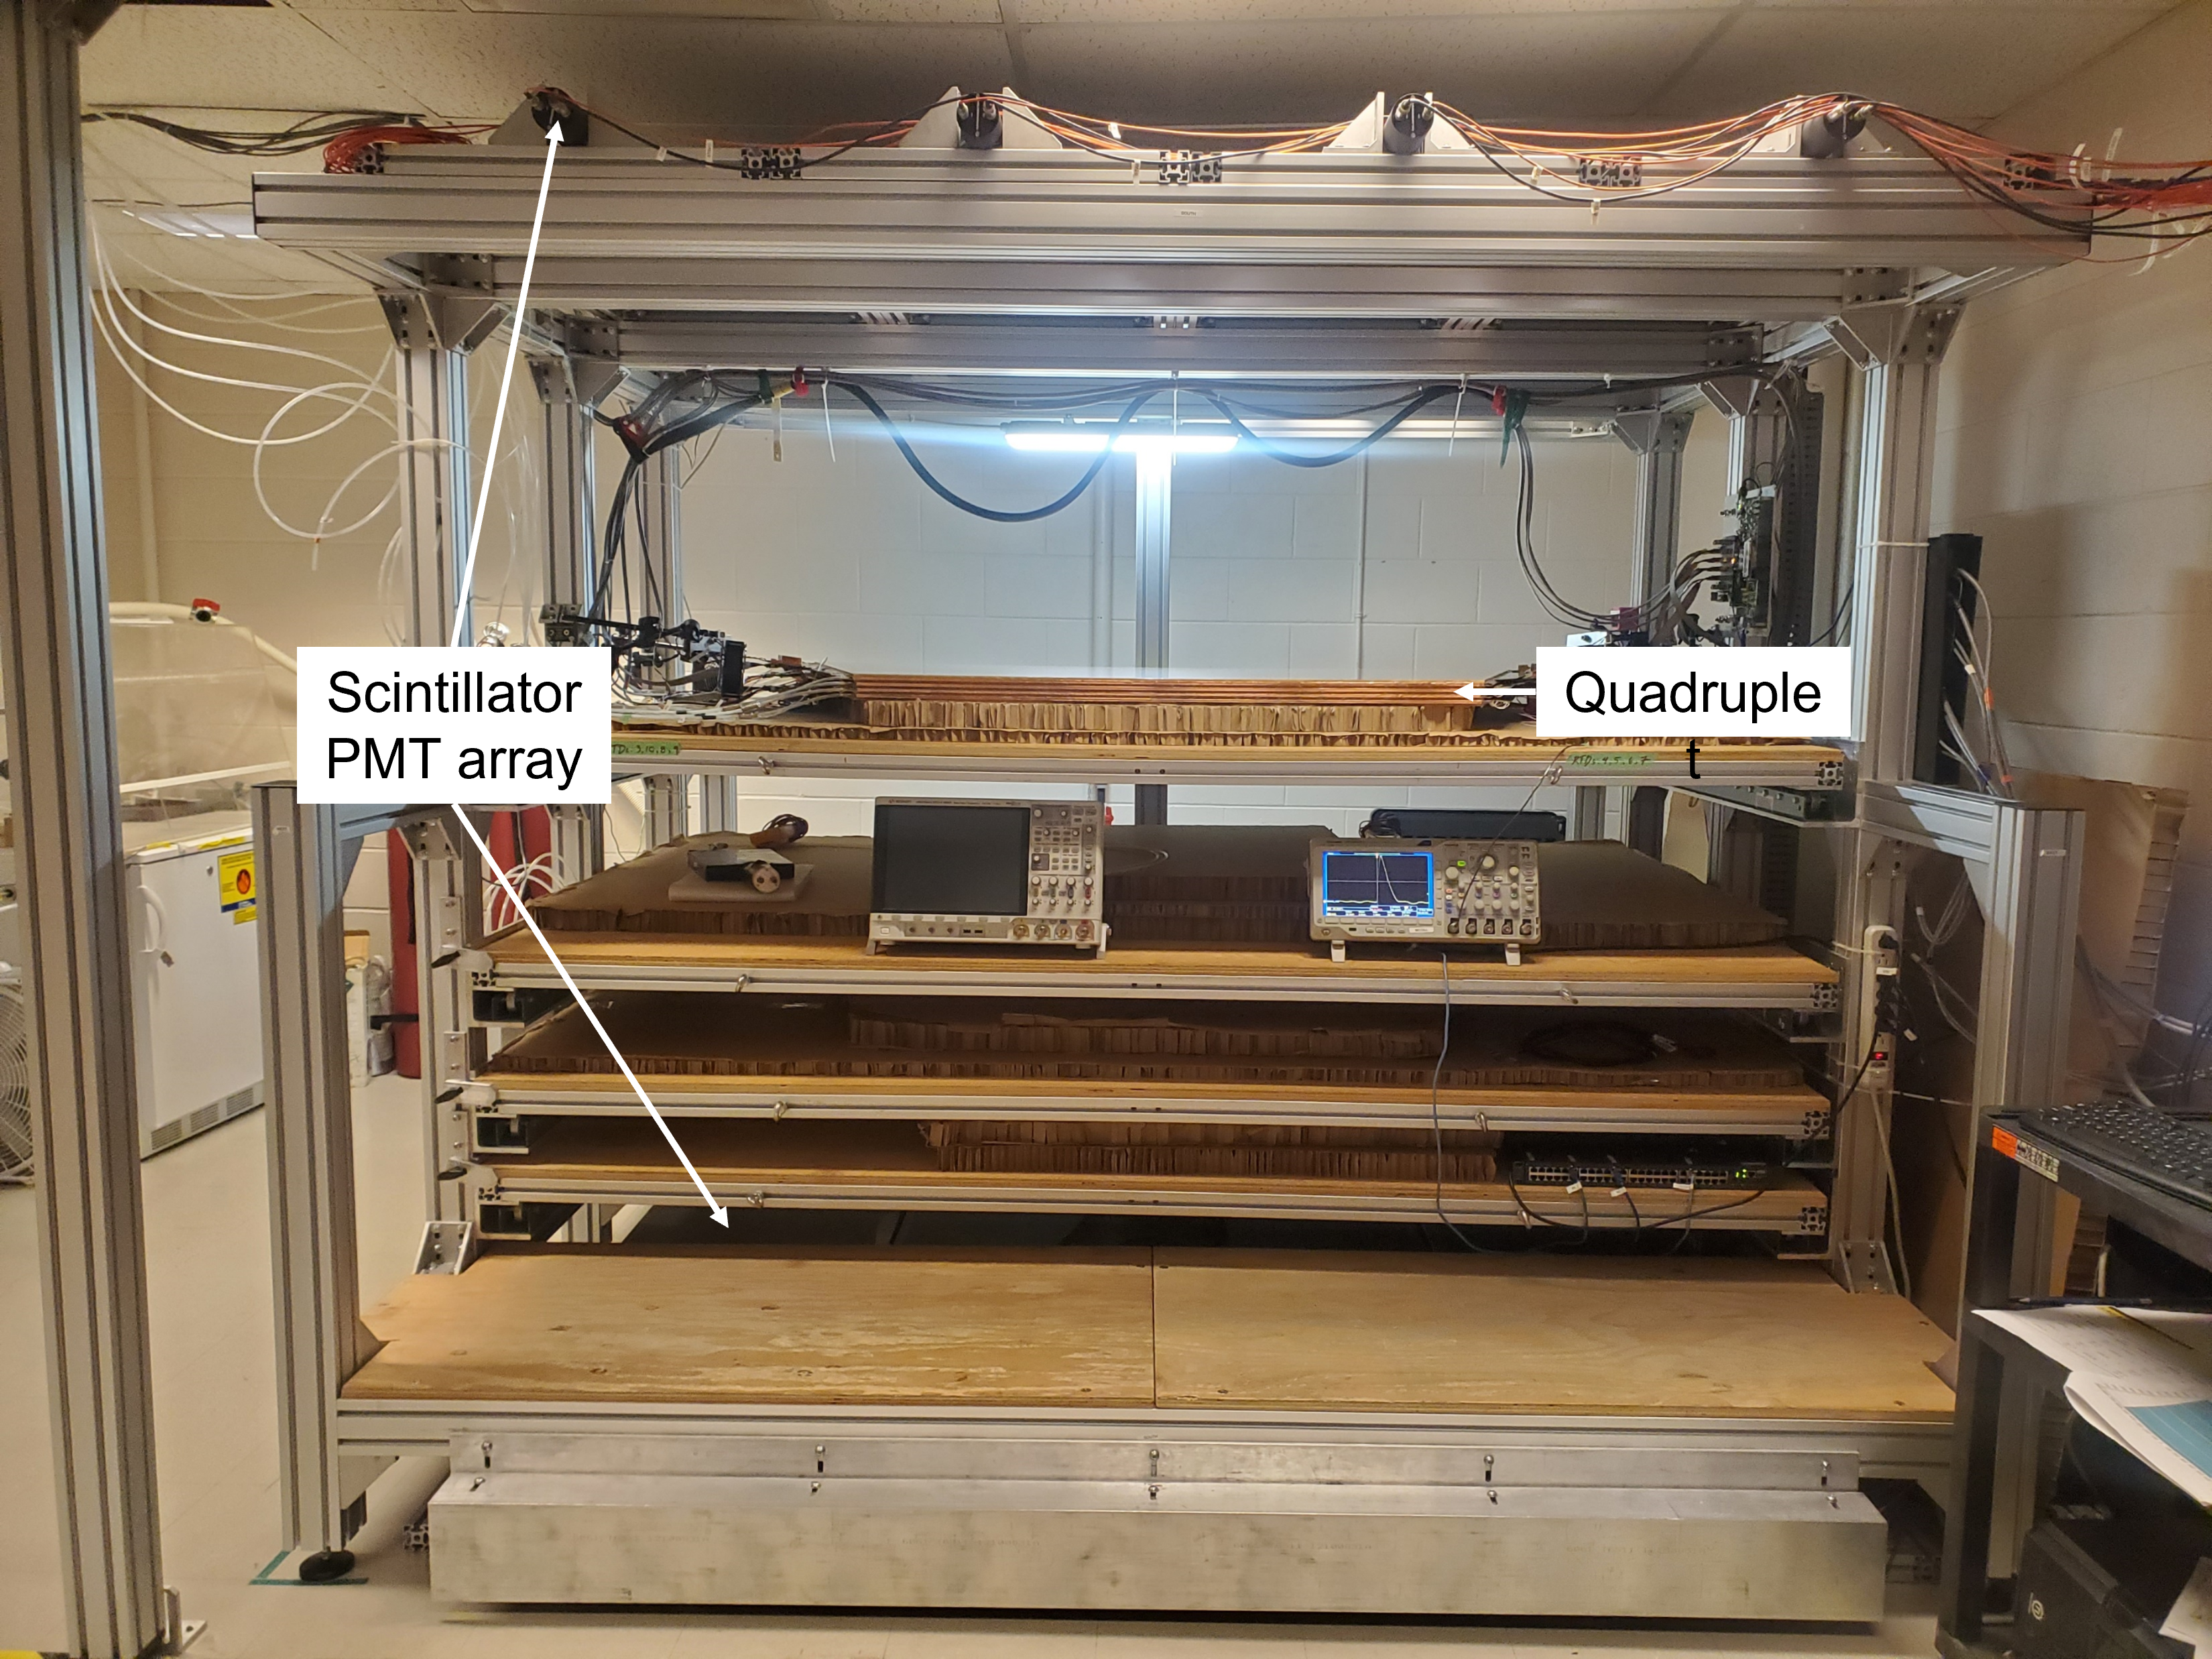
\includegraphics[width = 0.9\textwidth]{figures/figure_test_bench.png}
    \caption{Cosmic muon hodoscope at McGill University with sTGC quadruplet in position.}
    \label{fig:hodoscope}
\end{figure}

Each sTGC electrode was connected to a channel on a VMM3~\cite{iakovidis_vmm3_2017}, which was set to measure and record the peak detector output (PDO) and the time at which that ouput occured (TDO) \textcolor{red}{if the channel was above threshold} (set by the configuration/readout software~\cite{siyuan_sun_stgc_readout_sw}).
QUICK: for each trigger, all PDO and TDO values (more?) were recorded and stored by the readoutsoftware into a binary file which was decoded into a usable root tree by the DECODER (CITE). Neighbour logic for strips. Then clustering.
    
%TODO : Mention slow control and gas system where?